\chapter{Nuclear shape effects on the bound-electron $\maybebm{g}$~factor}
\label{ch:nucl_def}

In this chapter, non-perturbative calculations of the nuclear deformation (ND) correction to the bound-electron $g$~factor are presented. Results for nuclei across the entire nuclear chart are shown, quantifying the higher-order corrections in the values of the $g$~factor. Furthermore, it is shown how the model dependence and therefore uncertainty of the finite nuclear size correction can be reduced by using deformed nuclear charge distributions and that, in this connection, numerical calculations are necessary for obtaining precise results. A part of the work described in this chapter was submitted for publication in Ref.~\cite{michel_nuclDef}. In Sections \ref{sec:gfac_motiv}, \ref{sec:gfac_avpot}, and \ref{sec:gfac_intro}, a motivation and a brief summary of the theory for the bound-electron $g$~factor for spinless nuclei is given. In Section \ref{sec:gfac_shape}, the definition of the ND correction from Ref.~\cite{jacek2012} is given and the numerical approach for its calculation from this thesis is compared to the previously used perturbative method.

\section{Motivation}
\label{sec:gfac_motiv}
The electron's $g$~factor characterizes its magnetic moment in terms of its angular momentum. For an electron bound to an atomic nucleus, the $g$~factor can be predicted in the framework of bound-state quantum electrodynamics (QED) as well as measured in Penning traps, both with a very high degree of accuracy, e.g.~\cite{Sturm2014,Sturm2011}. This enables extraction of information on fundamental interactions, constants and nuclear structure. For example, the combination of theory and precise measurements of the bound electron $g$~factor has recently provided an improved value for the electron mass~\cite{Sturm2014}, and bound-state QED in strong fields was tested with unprecedented precision~\cite{Haffner2000, Verdu2004, Kohler2015, Zatorski2017}. It also enables measurements on characteristics of nuclei such as electric charge radii, as shown for $\textrm{Si}^{13+}$~\cite{Sturm2011}, or the isotopic mass difference as demonstrated for $\null^{48} \textrm{Ca}$ and $\null^{40} \textrm{Ca}$ in Ref.~\cite{Kohler2016}, or, as proposed theoretically, nuclear magnetic moments~\cite{Yerokhin2011}.  Also, it was argued that $g$-factor experiments with heavy ions could result in a independent determination of the fine-structure constant which is more accurate than the presently established one~\cite{Shabaev2006,yerokhin2016}.
With planned experiments involving high $Z$ nuclei~\cite{HITRAP2008,vogel2015,sturm2017} and current experimental accuracies on the $10^{-10}$ level for low $Z$, it is important to keep track also of higher-order effects. 
In this context, besides one-loop QED corrections~\cite{Yerokhin2004,yerokhin2017} which are well under control, two-loop QED~\cite{Pachucki2005,yerokhin2013,czarnecki2016,czarnecki2018} which requires further investigations, and nuclear polarization~\cite{Nefiodov,volotka2014}, also the influence of nuclear size~\cite{karshenboim2000,Glazov2002} and shape is critical.
In Refs.~\cite{jacek2012, ZatorskiWorkingNotes}, the nuclear shape correction to the bound-electron $g$~factor was introduced and calculated for spinless nuclei using the perturbative effective-radius method (ERM)~\cite{Shabaev1993,kozhedub2008}. This effect accounts for the influence of a deformed nuclear charge distribution and changes the $g$~factor up to a $10^{-6}$ level for heavy nuclei, thus being potentially important for future experiments.
Additionally, the uncertainty of the finite nuclear size correction to the Lamb shift in hydrogenlike $^{238}$U was shown to be sensitive on nuclear deformation effects~\cite{kozhedub2008}.
This motivates the possibility of a lowering of uncertainties for the $g$~factor by considering ND.
Therefore, a comparison of experiment and theory for heavy nuclei demands a further improvement and critical scrutiny of the validity of the previously used perturbative methods, as pointed out in Ref.~\cite{karshenboim2018}.

\section{Averaged Nuclear Potential}
\label{sec:gfac_avpot}
In this section, the electric interaction energy between a spinless atomic nucleus, described by a rigid rotor model (Appendix~\ref{app:rig_rotor}), and an electron in a hydrogen-like ion is investigated, following~\cite{kozhedub2008,jacek2012}. In Chapter~\ref{ch:furry_pic}, it was shown that to leading order the bound-state energies can be obtained by solving the Dirac equation for the electron in the nuclear potential. For a rigid rotor, the charge density $\rho(\mathbf{r}^{\prime}_N)$ is given in the nuclear body-fixed frame, and the position of the body fixed frame in the laboratory frame is described in terms of the Euler angles~$(\phi,\theta,\psi)$. In the following, primed coordinates refer to the body-fixed system and unprimed coordinates to the laboratory system, and vectors are written in spherical coordinates as $\mathbf{r}_i=(r_i,\vartheta_i,\varphi_i)$. The passive picture of rotations is used, i.e. the vectors are considered as invariant geometric objects and the Euler angles are used to describe the rotations of the coordinate axes. The electric potential energy of an electron at position $\mathbf{r}_{e}^\prime$ due to the nuclear electric field is
\begin{equation}
V(\mathbf{r}_e^\prime)=-Z\alpha \int\mathrm{d}^3\mathbf{r}_N^\prime\,
\frac{\rho(\mathbf{r}_N^\prime)}{\left|\mathbf{r}_e^\prime - \mathbf{r}_N^\prime\right|}.
\end{equation}
Now, the denominator is expanded in spherical multipoles~\cite{jackson1999} without any assumptions about the distance of nuclear charge distribution and electron, which results in radial distribution functions of the $l$-th multipoles, instead of the usual scaling $\sim 1/r^{l+1}$ . Hereby, the potential is rewritten as
\begin{equation}
V(\mathbf{r}_e^\prime)=\sum_{l=0}^\infty \sum_{m=-l}^l V_{lm}(\mathbf{r}_e^\prime)=-Z\alpha \sum_{l=0}^\infty \sum_{m=-l}^l
\int\mathrm{d}^3\mathbf{r}_N^{\prime}\,\frac{r_<^l}{r_>^{l+1}}\rho(\mathbf{r}_N^\prime) C_{lm}^*(\vartheta^\prime_N,\varphi_N^\prime) C_{lm}(\vartheta^\prime_e,\varphi_e^\prime),
\label{eq:mulitipoles_1}
\end{equation}
where $r_>=\max(r^\prime_N,r^\prime_e)$ and $r_<=\min(r^\prime_N,r^\prime_e)$, and $C_{lm}(\vartheta,\varphi)=\sqrt{4\pi/(2l+1)}Y_{lm}(\vartheta,\varphi)$ are the normalized spherical harmonics. Since the laboratory frame and the body fixed frame are related by a rotation, the absolute value of vectors stays the same, i.e. $r^\prime_i = r_i$.
%In the following, spinless nuclei are considered, which are axially symmetric with respect to the body-fixed $z^\prime$ axis, as most nuclei are~\cite{zickendraht1991}. As a consequence, only the $m=0$ terms of Eq.~\eqref{eq:mulitipoles_1} give a non-zero contribution.
Since the angular variables are separated by the multipole expansion, the electronic angles can be transformed to the laboratory system in a simple way, while keeping the nuclear variables in the body-fixed frame. The body-fixed variables $\vartheta^{\prime}_e,\varphi^\prime_e$ are in general a function of the laboratory $\vartheta_e,\varphi_e$ and the Euler angles~$(\phi,\theta,\psi)$. For the special case of spherical harmonics, the connection is
\begin{equation}
C_{l0}(\vartheta_e^\prime,\varphi_e^\prime) = \sum_{\tilde{m}=-l}^l C^{*}_{l\tilde{m}}(\theta,\phi)C_{l\tilde{m}}(\vartheta_e,\varphi_e).
\end{equation}
Furthermore, nuclear polarization effects~\cite{Nefiodov} are neglected, so it is assumed that the nucleus is in its ground state only and the interaction with the electron does not induce virtual nuclear transitions. This assumption is a valid approximation, since the typical nuclear energy scales are on the order of $100\,$keV, which is much larger than typical energies in atomic physics. Under these conditions, the nuclear degrees of freedom can be integrated out via the expectation value of the electric potential with the nuclear ground state wave functions, which correspond in the rigid rotor model to $I=M=K=0$. Due to the vanishing nuclear spin, only $l=m=\tilde{m}=0$ terms are non-zero, and the potential~\eqref{eq:mulitipoles_1} reduces to
\begin{alignat}{2}
\label{eq:gfac_monopole}
&V(r_e)&&=-Z\alpha \int\mathrm{d}^3\mathbf{r}^\prime_N\frac{\rho(\mathbf{r}_N^\prime)}{r_>}\\
& &&= -\frac{Z\alpha}{r_e} 4\pi\int_0^{r_e}\mathrm{d}r_N^\prime r_N^{\prime\,2}\rho_0(r_N^\prime) 
-Z\alpha 4\pi\int_{r_e}^\infty\mathrm{d}r_N^\prime r_N^{\prime}\rho_0(r_N^\prime), \notag
\end{alignat}
with the averaged charge distribution
\begin{equation}
\label{eq:rho_averaged}
4\pi\rho_0(r^\prime_N)=\int_0^{2\pi}\mathrm{d}\varphi_N^\prime \int_0^\pi \mathrm{d}\vartheta_N^\prime \sin\theta\,\rho(\mathbf{r}_N^\prime).
\end{equation}
Thus, for spinless nuclei, the potential is spherically symmetric, although the charge distribution of the nucleus does not have to be. Therefore, the theory of the bound-electron $g$ factor in a spherical potential can be applied also in this case.

\section{Bound-electron $\maybebm{g}$ factor in central potentials}
\label{sec:gfac_intro}
In the previous subsection, it was shown that for spinless nuclei the electric potential for a bound electron is still spherically symmetric, even for deformed nuclear charge distributions. Therefore, in this section, the theory of the $g$~factor in a spherically symmetric potential is presented, following~\cite{rose1961,Karshenboim2005}. A more detailed introduction can be found in Ref.~\cite{michel2015}. In a weak, homogeneous magnetic field, the $g$~factor is determined by the energy splitting, which is linear in the field strength. Therefore, an electron moving in an arbitrary central potential $V(r_e)$ of the nucleus and in a homogeneous magnetic field $\mathbf{B}$ is considered. The $z$ axis is aligned along the magnetic field, i.e. $\mathbf{B}=B\mathbf{e}_z$, where $\mathbf{A}(\mathbf{r})=\mathbf{B}\times \mathbf{r} /2$ is the corresponding vector potential in Coulomb gauge. The stationary Dirac equation for the electron thereby reads as
\begin{equation}
\left[\boldsymbol{\alpha}\cdot\mathbf{p}+\beta m_e + V(r) -e\boldsymbol{\alpha}\cdot\mathbf{A}(\mathbf{r})\right]\,\left|\psi\right> = E\,\left|\psi\right>.
\end{equation}
Since for the $g$ factor in a weak field only the energy splitting linear in the magnetic field strength is needed, it is enough to solve the Dirac equation with the nuclear potential as
\begin{equation}
\left[\boldsymbol{\alpha}\cdot\mathbf{p}+\beta m_e + V(r) \right]\,\left|n\kappa m\right> = E\,\left|n\kappa m\right>,
\end{equation}
where the methods for spherical potentials presented in Section~\ref{sec:sph_dirac} can be used. Then, the first order energy splitting due to the magnetic field is considered as
\begin{equation}
\Delta E_B = -e\left<n\kappa m\right|\boldsymbol{\alpha}\cdot\mathbf{A}(\mathbf{r})\left|n\kappa m\right>.
\label{eq:gfacmatel}
\end{equation}
Following Ref.~\cite{relativistic_electron_theory} for the calculation of the matrix element in Eq.~\eqref{eq:gfacmatel}, the energy splitting can be derived with angular momentum theory as $$\Delta E_B = m\, g \mu_B B,$$ where the $g$~factor is defined as the proportionality constant between energy shift and product of the quantum number $m$, Bohr magneton $\mu_B=|e|\hbar/(2m_e)$ and field strength~$B$ as
\begin{equation}
g=\frac{2m_e\kappa}{j(j+1)}\int_0^\infty\mathrm{d}r r^3 f_{n\kappa}(r)g_{n\kappa}(r).
\label{eq:gfac_central}
\end{equation}
It has been shown in Ref.~\cite{Karshenboim2005}, that the radial integral in Eq.~\eqref{eq:gfac_central} is related to the derivative of the electron energies with respect to its mass. As a first step, a transformation of the radial integral in Eq.~\eqref{eq:gfac_central} can be performed. For this, the first line of the radial equations~\eqref{eq:radial_equations_small} is multiplied by $g(r)$ and the second line is multiplied by $f(r)$. Then, the sum of these equation is independent of the energy $E$ and the potential $V(r)$ and by integrating this sum over $r$, the following identity of radial integrals is obtained:
\begin{equation}
\int\mathrm{d}r r^3 f(r)g(r) = -\frac{1}{4m_e}
\text{\huge(}1-2\kappa \int_0^\infty\mathrm{d}r r^2 (f(r)^2-g(r)^2)\text{\huge)}.
\end{equation}
Now, the radial integral on the right hand side can be expressed in terms of the expectation value of the $\beta$ matrix, using its definition from Appendix~\ref{app:conventions}, as
\begin{equation}
-\int_0^\infty\mathrm{d}r r^2 (f(r)^2-g(r)^2)=\left<n\kappa m\middle|\beta\middle|n\kappa m\right>
\end{equation}
Since for potentials which do not depend on the mass of the electron, $\beta$ can be expressed by the derivative of the Dirac Hamiltonian~\eqref{eq:sphdirac} as $\beta = \partial\text{H}_D/\partial m_e$, it follows that
\begin{equation}
\left<n\kappa m\right|\beta\left|n\kappa m\right> = \left<n\kappa m\right|\partial\text{H}_D/\partial m_e\left|n\kappa m\right> = \partial E_{n\kappa}/\partial m_e,
\end{equation}
and the $g$~factor~\eqref{eq:gfac_central} can be written as
\begin{equation}
g = \frac{-\kappa}{j(j+1)}\left( 1-2\kappa\frac{\partial E_{n\kappa}}{\partial m_e}\right).
\label{eq:gfac_viaDeriv}
\end{equation}
This formula is valid for arbitrary central potentials and can be used for numerical and analytical calculations. Using the expression for the energies in the pure Coulomb potential from Eq.~\eqref{eq:finestructure_formula}, the ground state $g$~factor for a point-like nucleus with charge number $Z$ reads as
\begin{equation}
\label{eq:point_gfac}
g_{\text{Point}}=\frac{2}{3}\left( 1+2\sqrt{1-(Z\alpha)^2}\right),
\end{equation}
a result which can also be obtained by integration of Eq.~\eqref{eq:gfac_central} with the known Coulomb wave functions and was reported first by Breit~\cite{breit1928}.

The resulting bound-electron $g$~factor differs from the point-like value~\eqref{eq:point_gfac} for an extended nuclear charge distribution. Correspondingly, the finite nuclear size correction is defined as the difference between the $g$~factor of the extended charge distribution~\eqref{eq:gfac_viaDeriv} and for the point-like nucleus as
\begin{equation}
\delta g_{\text{FS}}=g-g_{\text{Point}}.
\end{equation}
%
%chare distribution figure start
\begin{figure*}
\centering
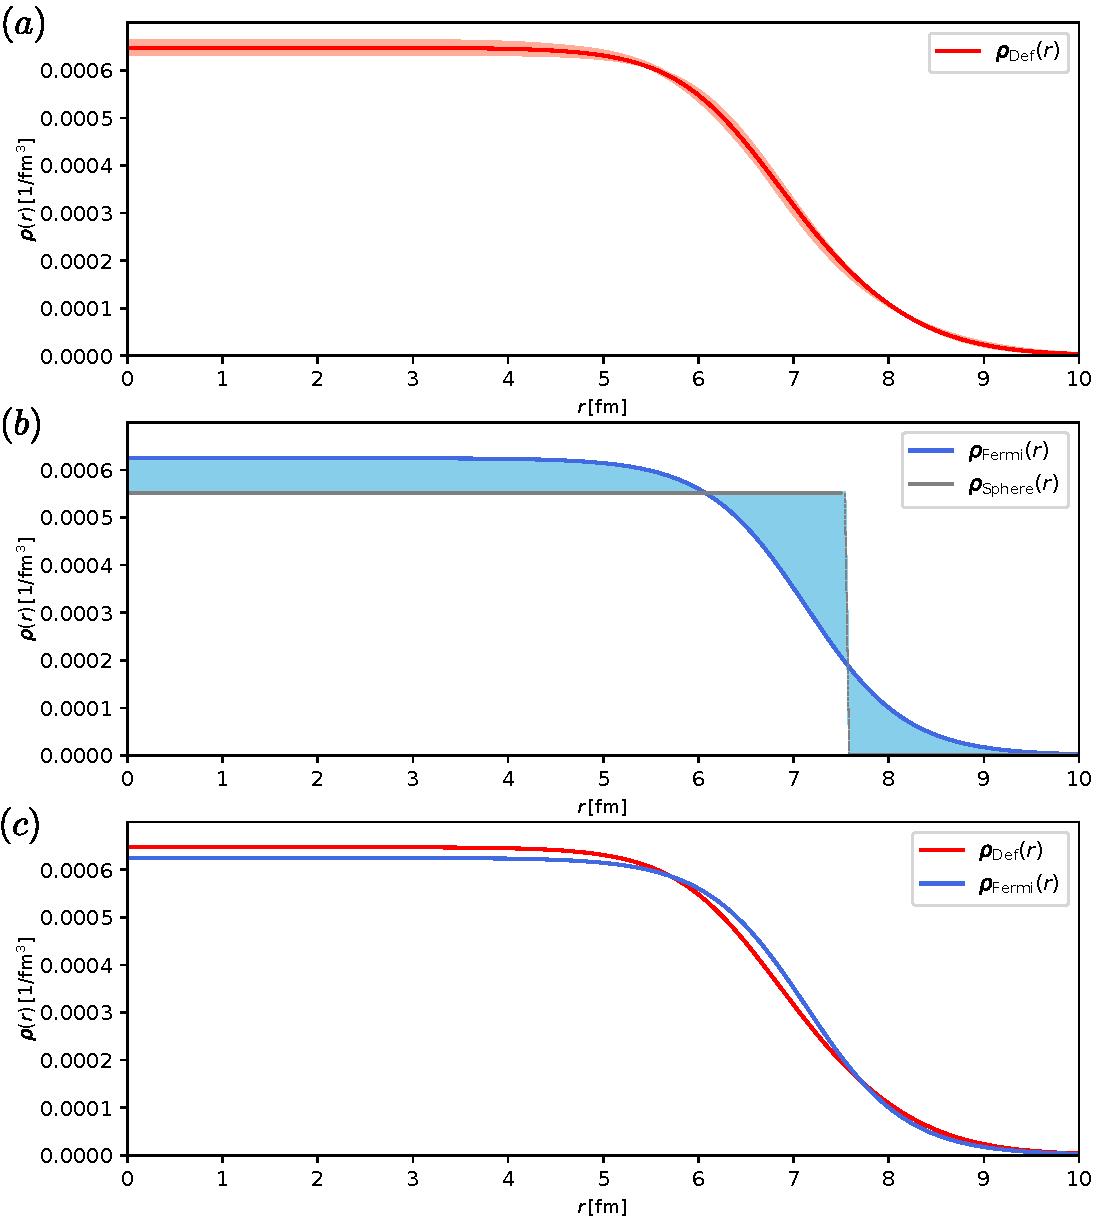
\includegraphics[width=\textwidth]{pics/chargeDistr2.pdf}\\
\caption{\label{fig:charge distr.}\\
(a): Averaged deformed Fermi distribution from Eq.~\eqref{eq:rho_averaged} for $^{238}$U, where the parameters and their uncertainties are taken from~\cite{jacek2012}. The light red band shows the uncertainties due to the parameters $a$, $\beta_2$, $\beta_4$, which is the remaining model uncertainty once the nuclear charge radius is fixed.\\
(b): (Non-deformed) Fermi distribution and homogeneously charged sphere with the same RMS charge radius as the deformed Fermi distribution. The difference (in light blue) is the conventional model uncertainty of the unclear charge distribution, which is larger compared to using the deformed Fermi distribution in subfigure a).\\
(c): Comparison of non-deformed and averaged, deformed Fermi distribution with the same RMS radius. The difference causes the nuclear deformation effect.}
\end{figure*}
% charge distribution figure end
%
\section{Non-perturbative analysis of nuclear shape effects}
\label{sec:gfac_shape}
In this work, we focus on quadrupole deformations and beyond, since atomic nuclei do not possess static dipole moments. Here, the deformed Fermi distribution
\begin{equation}
\rho_{ca\beta_2\beta_4}(r,\vartheta)=N\left[1+\text{exp}\left(\frac{r-c(1+\beta_2 \text{Y}_{20}(\vartheta)+\beta_4 \text{Y}_{40}(\vartheta))}{a}\right)\right]^{-1}
\label{eq:deffermi}
\end{equation}
as a model of the nuclear charge distribution has proved to be very successful, e.g. in heavy muonic atom spectroscopy with deformed nuclei \cite{hitlin1970,tanaka1984}. The normal Fermi distribution (${\beta_i}{=}{0}$) has also been used in electron-nucleus scattering experiments determining the nuclear charge distribution \cite{hahn1956}. Here, $a$ is a skin thickness parameter and $c$ the half-density radius, while $\beta_2$, $\beta_4$ are deformation parameters. The $\text{Y}_{lm}(\vartheta,\varphi)$ are the spherical harmonics and the $\text{Y}_{l0}(\vartheta)$ depend only on the polar angle~$\vartheta$, and not on the azimuthal angle~$\varphi$. The normalization constant $N$ is determined by the condition
\begin{equation}
\int \text{d}^3r\, \rho_{ca\beta_2\beta_4}(r,\vartheta)=1.
\end{equation}%
For the deformed Fermi distribution~\eqref{eq:deffermi} with a fixed charge number $Z$, the $g$~factor~\eqref{eq:gfac_central} is completely determined by the parameters $c$, $a$ and $\beta_i$, and therefore can be written for the ground state as
\begin{equation}
g = g_{\text{point}} + \delta g^{(ca\beta_2\beta_4)}_{\text{FS}},
\label{eq:finiteDef}
\end{equation}
where $\delta g^{(ca\beta_2\beta_4)}_{\text{FS}}$ is the finite-size correction depending on the parameters $c$, $a$, and $\beta_i$. In Ref.~\cite{jacek2012}, the ND correction to the bound electron $g$~factor has been defined as the difference of the finite size effect due to a deformed charge distribution and due to a symmetric charge distribution (i.e. ${\beta_i}{=}{0}$) with the same nuclear RMS radius as
\begin{equation}
\delta g_{\text{ND}}=\delta g^{(c_1a\beta_2\beta_4)}_{\text{FS}} - \delta g^{(c_2a00)}_{\text{FS}},
\label{eq:defdgnd}
\end{equation}
where $a\approx 2.3\,\text{fm}/(4\text{ln}(3))$, and $c_i$ are determined such that $\sqrt{\left<r^2\right>_{\rho}}$ of the corresponding charge distribution agrees with the root-mean-square (RMS) values determined experimentally~\cite{Angeli2013}. The $n$-th moment of a charge distribution $\rho(\mathbf{r})$ is defined as
\begin{equation}
\left< r^n \right>_{\rho} = \int \text{d}^3\mathbf{r}\,\, r^n \rho(\mathbf{r}).
\label{eq:nmoment}
\end{equation}
Values for the deformation parameter $\beta_2$ can be obtained from literature values of the reduced electric quadrupole ($E2$) transition probabilities from a nuclear state $2^+_i$ to the ground state $0^+$ via~\cite{Trager}
\begin{equation}
\beta_2 = \frac{4\pi}{3Z|e|\sqrt{5\left< r^2\right>_{\rho} /3}}\left[ \sum_i B(E2;0^+\rightarrow 2_i^+) \right]^{1/2},
\label{eq:beta}
\end{equation}
and estimates for $\beta_4$ can be found e.g. in Ref.~\cite{Moller1995}.
From Eq.~\eqref{eq:defdgnd} it is evident that the ND correction is a difference of two finite-size effects and therefore especially sensitive to higher order effects. For high $Z$ it reaches the $10^{-6}$~level and therefore it is very significant.

In Ref.~\cite{jacek2012}, $\delta g_{\text{FS}}^{(ca\beta_2\beta_4)}$ and $\delta g_{\text{ND}}$ were calculated with the ERM~\cite{Shabaev1993}. It was shown that these mainly depend on the moments $\left< r^2 \right>_{\rho}$ and $\left< r^4 \right>_{\rho}$ from Eq.~\eqref{eq:nmoment}.
$\delta g_{\text{ND}}$ can be calculated with the formula~\cite{Karshenboim2005}
\begin{equation}
\delta g^{(ca\beta_2\beta_4)}_{\text{FS}}=\frac{4}{3}\frac{\partial E_{\text{FS}}(c,a,\beta)}{\partial m_e},
\label{eq:effrad}
\end{equation}
which is a direct consequence of Eq.~\eqref{eq:gfac_viaDeriv} and where $E_{\text{FS}}(c,a,\beta_2,\beta_4)$ is the energy correction due to $\rho_{ca\beta_2\beta_4}(r,\vartheta)$ compared to the point-like nucleus.

The effective radius~$R$ is defined as the radius of a homogeneously charged sphere with the same energy correction $E^{(\text{sph})}_{\text{FS}}(R)$ as the deformed Fermi distribution via
\begin{equation}
E^{(\text{sph})}_{\text{FS}}(R) \equiv E_{\text{FS}}(c,a,\beta_2,\beta_4).
\label{eq:effradNum}
\end{equation}
The energy correction can be approximated~\cite{Shabaev1993} as
\begin{equation}
E^{(\text{sph})}_{\text{FS}}(R)\approx\frac{(Z\alpha)^2}{10}\left[{1}{+}(Z\alpha)^2f(Z\alpha) \right](2Z\alpha R m_e)^{2\gamma}m_e.
\label{eq:efs}
\end{equation}
Here, $f(x)=1.380-0.162x+1.612x^2$ and the effective radius is approximately
\small
\begin{equation}
R\approx\sqrt{\frac{5}{3}\left<r^2\right>_{\rho_{ca\beta_2\beta_4}}\left[ 1-\frac{3}{4}(Z\alpha)^2 \left( \frac{3}{25}\cfrac{\left<r^4\right>_{\rho_{ca\beta_2\beta_4}}}{\left<r^2\right>^2_{\rho_{ca\beta_2\beta_4}}}-\frac{1}{7} \right) \right]}.
\label{eq:radius}
\end{equation}
\normalsize
While Eq.~\eqref{eq:effrad} is exact for an arbitrary central potential, provided that $E_{\text{FS}}$ is known exactly, Eq.~\eqref{eq:efs} is an approximation derived under the assumption of the difference between point-like and extended potential being a small perturbation. The calculation of the ND correction to the $g$~factor via the effective radius approach therefore relies on a perturbative evaluation of the energy derivative in Eq.~\eqref{eq:effrad} and is limited by the accuracy of the finite-size corrections.

In this work, the ND $g$-factor correction is calculated with three methods. 
Firstly, with the previously used analytical ERM described above. Secondly, with a numerical ERM, where instead of the approximative Eqs.~\eqref{eq:efs} and \eqref{eq:radius}, Eq.~\eqref{eq:effradNum} is solved numerically for $R$ and the ND $g$-factor correction is obtained by using Eq.~\eqref{eq:gfac_central} with the wave functions of the corresponding charged sphere.
Finally, we also calculate $\delta g_{\text{ND}}$ non-perturbatively by solving the Dirac equation~\eqref{eq:diracSph} numerically with the dual-kinetic-balance method~\cite{dualkinetic} for the potential \eqref{eq:gfac_monopole}, including all finite size effects due to the deformed charge distribution $\rho_{ca\beta}(r,\vartheta)$. Then, the $g$~factors in Eq.~\eqref{eq:defdgnd} for the ND correction can be obtained by numerical integration of the wave functions in Eq.~\eqref{eq:gfac_central}. Alternatively, the derivative of the energies in Eq.~\eqref{eq:gfac_viaDeriv} can be calculated numerically as 
\begin{equation}
\frac{\partial E_{n\kappa}}{\partial m_e} \approx \frac{E_{n\kappa}^{(m_e+\delta m_e)}-E_{n\kappa}^{(m_e-\delta m_e)}}{2 \delta m_e},
\end{equation}
with a suitable ${\delta m_e / m_e}{\ll}{1}$, since the uncertainty of the numerical derivative scales as $(\delta m_e/m_e)^3$. Here, $E_{n\kappa}^{(m_i)}$ stands for the binding energy obtained by solving the Dirac equation with the electron mass replaced by $m_i$. Both methods were found to be in excellent agreement.

\begin{figure*}
  \centering
  \begin{minipage}[b]{\textwidth}
    \centering
    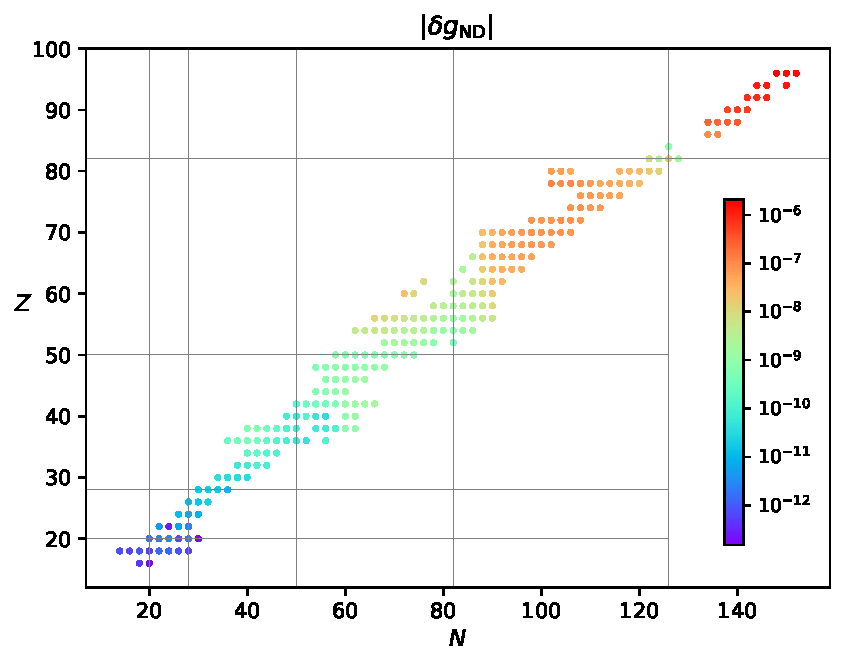
\includegraphics[width=\textwidth]{pics/dgnuclchart.pdf}\\
    \caption{\label{fig:dg}Nuclear chart with charge number $Z$ and neutron number $N$, where the grey lines indicate the magic numbers 20, 28, 50, 82, and 126. The points represent even-even nuclei, where their color displays the magnitude of the ND $g$-factor correction $\delta g_{\text{ND}}$, calculated with the numerical, non-perturbative approach, which takes particularly low values around the magic numbers and larger values in between. See~\cite{michel2015} for an evaluation with the previously used perturbative method.}
  \end{minipage}
\end{figure*}

The ND $g$-factor correction was calculated for a wide range of even-even, both in the proton and neutron number, and therefore spinless nuclei with charge numbers between 16 and 96 using the deformed Fermi distribution from~Eq.~\eqref{eq:deffermi} with parameters $a$, $c$, and $\beta$ obtained as described below Eq.~\eqref{eq:defdgnd}. The required RMS values for the nuclear charge radius are taken from~\cite{Angeli2013} and the reduced transition probabilities needed for the calculation of $\beta_2$ via Eq.~\eqref{eq:beta} from Ref.~\cite{ENSDF}. The resulting values for $|\delta g_{\text{ND}}|$, obtained by the non-perturbative method, are shown in Fig.~\ref{fig:dg} as a function of the charge number $Z$ and the neutron number $N$. If the proton or neutron number is in the proximity of a nuclear magic number 2, 8, 20, 28, 50, 82, and 126, which corresponds to a filled proton or neutron shell \cite{Ring}, the nuclear shell-closure effects also transfer to the $g$~factor, and the ND correction is reduced, as already indicated with the perturbative ERM method in Ref.~\cite{michel2015}. In Table~\ref{tab:spline}, a comparison between all our numerical approaches and the analytical ERM results from \cite{jacek2012} is shown.

Now, let us discuss the main sources for the disagreement of the results obtained with the different approaches, as presented in Table~\ref{tab:spline}. Both Eqs.~\eqref{eq:efs} and~\eqref{eq:radius} are approximations derived by perturbation theory, which affects the accuracy of the analytical ERM $\delta g_{\text{ND}}^{(\text{eff,A})}$. Eq.~\eqref{eq:efs} has an estimated relative uncertainty ${\scriptstyle\lesssim}\,0.2\,\%$~\cite{Shabaev1993} and \eqref{eq:radius} uses only the second and fourth moment of the nuclear charge distribution for finding the effective radius. Also, it was shown in Ref.~\cite{karshenboim2018} that the analytical ERM for arbitrary charge distributions is incomplete in order $(Z\alpha)^2m_e(Z\alpha m_e R_N)^3$, where $R_N$ is the nuclear RMS charge radius. Furthermore, even if the effective radius is calculated without approximations according to Eq.~\eqref{eq:effradNum}, the wave functions of the corresponding homogeneously charged sphere slightly differ from the ones of the deformed Fermi distribution with the same binding energy. This affects values of the $g$~factor and explains the difference between the numerical ERM $\delta g_{\text{ND}}^{(\text{eff,N})}$ and the direct numerical calculations $\delta g_{\text{ND}}^{(\text{num})}$. 
Finally, being a difference of two small finite-nuclear-size corrections, the ND correction can exhibit enhanced sensitivity on the uncertainty of the ERM.
From Table~\ref{tab:spline}, one can conclude that for high $Z$, the difference between analytical ERM and non-perturbative calculations is mainly due to the approximations in Eqs.~\eqref{eq:efs} and~\eqref{eq:radius}. The analytical ERM proved to be a good order-of-magnitude estimate of the ND correction, but for high-precision calculations, non-perturbative methods beyond the ERM and without any expansion in $(Z\alpha)$ or $(Z\alpha\, m_e\, R_N)$ are indispensable. Convergence of the numerical methods was checked by varying numerical parameters and using different grids, and the obtained accuracy permits the consideration of nuclear size and shape with an accuracy level much higher than the differences to the perturbative method for the considered nuclei. For low-$Z$ nuclei, however, it becomes increasingly difficult to resolve the small deformation effect with numerical methods. Using double-precision arithmetics, in best case there are 15 to 16 relevant digits in a stored float. Therefore, the small corrections below the $10^{-16}$ level for light nuclei can not be resolved. On the other hand, for heavy nuclei the corrections on the $10^{-6}$ level can be easily seen with double-precision accuracy.\\

In summary, the ND $g$-factor correction was calculated non-perturbatively for a wide range of nuclei with quadrupole deformations estimated from nuclear data.
By comparing the previously used perturbative ERM and the all-order numerical approach, it was shown that the perturbative ERM overestimates the nuclear deformation correction up to the $20\,\%$ level.
In the low-$Z$ regime, the ND corrections can safely be neglected, especially for the ions considered in Ref.~\cite{Sturm2014}. However, considering a ND correction up to the parts-per-million level and an expected parts-per-billion accuracy, or even below, for the $g$-factor experiments with high-$Z$ nuclei, in this case an all-order treatment is indispensable. 
On the other hand, since the distribution of electric charge inside the nucleus is a major theoretical uncertainty for $g$~factors with heavy nuclei, the extraction of information thereon from experiments is possible. Once QED corrections are known to the required precision, this work demonstrates the required accurate mapping of arbitrary nuclear charge distributions to corresponding $g$~factors.\\[0.6cm]

\subsection{Reduction of model uncertainty of the finite size $\maybebm{g}$-factor correction}
In this part, the connection between nuclear finite size and nuclear deformation correction to the bound-electron $g$~factor is discussed in more detail, since these contributions are intertwined. It is not possible to calculate a value and uncertainty of one of these contribution independently of the other.

Without the consideration of a deformed charge distribution, commonly a non-deformed Fermi distribution (Eq.~\eqref{eq:deffermi} with ${\beta_2}{=}{\beta_4}{=}0$) which agrees with the RMS radius from literature is used to calculate the finite nuclear size correction. 
The uncertainty is due to the error in the RMS literature value and also due to model dependence, since even for a fixed RMS value and charge number, there are residual degrees of freedom in the charge distribution. The uncertainty due to the RMS value can be easily calculated. The uncertainty due to the model dependence is because of the difference between the Fermi distribution and the true, unknown nuclear charge distribution and is not so easy to estimate. The uncertainty due to model dependence is often estimated as the difference between the effects due to a Fermi distribution and a homogeneously charged sphere, which is considered to be a very conservative estimate~\cite{Shabaev2006}.

If the finite size correction is calculated as $\delta g^{(ca\beta_2\beta_4)}_{\text{FS}}$ from Eq.~\eqref{eq:finiteDef}, finite size and deformation effects are already included. Usually, the value of $c$ is determined by the RMS radius from literature. The remaining model uncertainty is reduced to the difference between the deformed Fermi distribution and the true, unknown nuclear charge distribution. As a consequence, precise values for the remaining parameters $a$, $\beta_2$ and $\beta_4$ need to be known, e.g. from muonic atom spectroscopy~\cite{Close1978,hitlin1970}. Furthermore, a reliable estimate of their error bars is needed for the estimate of the difference between deformed Fermi and the true charge distribution. In practice, this leads to a reduced model uncertainty due to the more realistic model of the nuclear charge distribution.

The nuclear deformation effect from Eq.~\eqref{eq:defdgnd} was defined in Ref.~\cite{jacek2012} as the difference of a deformed ($\beta_i \neq 0$) and a normal Fermi distribution ($\beta_i=0$) for the \textit{same value} of $a$ and the RMS radius. 
Therefore, the nuclear deformation correction was defined in a model-dependent way, which requires a fixed model for the finite nuclear size correction. As a consequence, the uncertainties of these contributions are not independent. 
However, for comparison of theoretical and measured values of the $g$~factor, the sum of nuclear finite size and deformation effect is needed. Therefore, an estimation of uncertainties is best performed for $\delta g^{(ca\beta_2\beta_4)}_{\text{FS}}$, which includes both finite size and deformation.
 
The reduction of model uncertainties is demonstrated in Fig~\ref{fig:charge distr.}. Here, the averaged charge distribution for the deformed Fermi distribution for $^{238}$U with parameters from~\cite{jacek2012} is shown along with error bars due to the uncertainties in $a$, $c$, $\beta_2$, and $\beta_4$ also according to Ref.~\cite{jacek2012}. For comparison, the conventional way of estimating the model dependence is also demonstrated by showing the difference between the non-deformed Fermi and charged-sphere charge distribution.

Furthermore, the reduced uncertainties due to consideration of deformation effects are shown for $^{238}$U in Table~\ref{tab:uranium}. Parameters and their uncertainties for the RMS radius, $a$, $\beta_2$, and $\beta_4$ from Ref.~\cite{kozhedub2008} are used. The uncertainty of the finite size $g$~factor correction due to model dependence is reduced by about a factor of 7. Now, the RMS radius error is responsible for the largest part of the total uncertainty.  
In addition, Table~\ref{tab:uranium} shows that the difference of the ERM and the all-order numerical method is larger than the uncertainty due to nuclear parameters.
%
% begin table with model dependence
\begin{table}[t]
\caption{\label{tab:uranium}%
Comparison of the finite nuclear size $g$-factor correction for the (non-deformed) Fermi distribution $\delta g_{\text{FS}}^{(c_1a00)}$ and the deformed Fermi distribution $\delta g^{(c_2 a \beta_2\beta_4)}_{\text{FS}}$ for $^{238}$U, evaluated with the effective-radius method (eff. radius) and numerically. The numbers in the first and second parenthesis are the uncertainty due to the RMS charge radius and the model uncertainty, respectively. Parameters and their uncertainties were taken from Ref.~\cite{jacek2012}. The results show that considering a deformed charge distribution can significantly reduce the model uncertainty. Furthermore it demonstrates that our numerical method needs to be used for precise calculations. 
}
\centering
\begin{tabular}{l|cc}
&eff. radius&numerical\\\hline\\
%$old \delta g_{\text{FS}}^{\text{(Fermi)}}$&$1.2860(11)(31)\times 10^{-3}$&$1.2739(11)(25)\times 10^{-3}$\\[0.4cm]
%$old\delta g^{(ca\beta_2\beta_4)}_{\text{FS}}$&$1.2852(11)(9)\phantom{0}\times 10^{-3}$&$1.2733(11)(7)\phantom{0}\times 10^{-3}$\\[0.8cm]
$\delta g_{\text{FS}}^{(c_1a00)}$&$1.2842(23)(29)\times 10^{-3}$&$1.2722(23)(23)\times 10^{-3}$\\[0.4cm]
$\delta g^{(c_2a\beta_2\beta_4)}_{\text{FS}}$&$1.2829(23)(4)\phantom{0}\times 10^{-3}$&$1.2711(23)(3)\phantom{0}\times 10^{-3}$
\end{tabular}
\end{table}
%
% begin table with comarison non-pert vs. eff-rad
\begin{table}
\begin{minipage}{1.1\textwidth}
\caption{\label{tab:spline}%
Comparison of the nuclear deformation $g$~factor correction obtained by the effective-radius method (ERM) with the analytical expressions from Eqs.~\eqref{eq:efs} and~\eqref{eq:radius} ($\delta g_{\text{ND}}^{(\text{eff,A})}$), by the ERM with effective radius and corresponding energy correction calculated numerically ($\delta g_{\text{ND}}^{(\text{eff,N})}$) and non-perturbatively by direct numerical calculations ($\delta g_{\text{ND}}^{(\text{num})}$) for several isotopes. $R_N$ is the RMS nuclear electric charge radius from literature \cite{Angeli2013} and $\beta_2$, $\beta_4$ are the deformation parameters of the deformed Fermi distribution~\eqref{eq:deffermi}. The parameters of the deformed Fermi distribution were either taken from Ref.~\cite{jacek2012} or calculated as described in the text, where the $\beta_4$ values from Ref.~\cite{Moller1995} were used.
}
\centering
\renewcommand*{\thefootnote}{\alph{footnote}}
\begin{tabular}{lcccccc}
 & \multicolumn{1}{c}{$R{\scriptstyle _N(\text{fm})}$} & \multicolumn{1}{c}{$\beta_2$} & \multicolumn{1}{c}{$\beta_4$} & \multicolumn{1}{c}{$\delta g_{\text{ND}}^{(\text{eff,A})}$} & \multicolumn{1}{c}{$\delta g_{\text{ND}}^{(\text{eff,N})}$} & \multicolumn{1}{c}{$\delta g_{\text{ND}}^{(\text{num})}$}\\
\hline\\[-5pt]
$^{\phantom{0}58}_{\phantom{0}26}$Fe$\;$\footnotemark[1] & 3.775 & 0.274                 & -0.019        & $-2.10\times 10^{-11}$ & $-1.95\times 10^{-11}$ & $-1.99\times 10^{-11}$ \\[4pt]
$^{\phantom{0}82}_{\phantom{0}38}$Sr$\;$\footnotemark[1] & 4.248 & 0.263                 & 0.001         & $-3.57\times 10^{-10}$ & $-3.16\times 10^{-10}$ & $-3.27\times 10^{-10}$ \\[4pt]
$^{\phantom{0}86}_{\phantom{0}38}$Sr$\;$\footnotemark[2] & 4.226 & 0.134\footnotemark[3] & 0.000         & $-8.98\times 10^{-11}$ & $-8.01\times 10^{-11}$ & $-8.24\times 10^{-11}$ \\[4pt]
$^{100}_{\phantom{0}38}$Sr$\;$\footnotemark[2]           & 4.487 & 0.435\footnotemark[3] & 0.000         & $-1.08\times 10^{-09}$ & $-0.97\times 10^{-09}$ & $-1.00\times 10^{-09}$ \\[4pt]
$^{\phantom{0}98}_{\phantom{0}44}$Ru$\;$\footnotemark[1] & 4.423 & 0.194                 & 0.038         & $-6.91\times 10^{-10}$ & $-6.02\times 10^{-10}$ & $-6.21\times 10^{-10}$ \\[4pt]
$^{116}_{\phantom{0}48}$Cd$\;$\footnotemark[1]           & 4.620 & 0.190                 & -0.038        & $-1.13\times 10^{-09}$ & $-0.99\times 10^{-09}$ & $-1.02\times 10^{-09}$ \\[4pt]
$^{116}_{\phantom{0}50}$Sn$\;$\footnotemark[1]           & 4.625 & 0.108                 & -0.008        & $-5.03\times 10^{-10}$ & $-4.36\times 10^{-10}$ & $-4.48\times 10^{-10}$ \\[4pt]
$^{134}_{\phantom{0}54}$Xe$\;$\footnotemark[1]           & 4.790 & 0.113                 & 0.000         & $-1.09\times 10^{-09}$ & $-0.94\times 10^{-09}$ & $-0.96\times 10^{-09}$ \\[4pt]
$^{142}_{\phantom{0}60}$Nd$\;$\footnotemark[2]           & 4.912 & 0.100                 & 0.000         & $-2.01\times 10^{-09}$ & $-1.71\times 10^{-09}$ & $-1.76\times 10^{-09}$ \\[4pt]
$^{150}_{\phantom{0}60}$Nd$\;$\footnotemark[2]           & 5.042 & 0.278                 & 0.000         & $-1.70\times 10^{-08}$ & $-1.45\times 10^{-08}$ & $-1.49\times 10^{-08}$ \\[4pt]
$^{144}_{\phantom{0}62}$Sm$\;$\footnotemark[2]           & 4.945 & 0.090                 & 0.000         & $-2.14\times 10^{-09}$ & $-1.81\times 10^{-09}$ & $-1.85\times 10^{-09}$ \\[4pt]
$^{154}_{\phantom{0}62}$Sm$\;$\footnotemark[2]           & 5.111 & 0.328                 & 0.000         & $-3.24\times 10^{-08}$ & $-2.75\times 10^{-08}$ & $-2.82\times 10^{-08}$ \\[4pt]
$^{152}_{\phantom{0}64}$Gd$\;$\footnotemark[1]           & 5.077 & 0.202                 & 0.050         & $-1.86\times 10^{-08}$ & $-1.56\times 10^{-08}$ & $-1.60\times 10^{-08}$ \\[4pt]
$^{208}_{\phantom{0}82}$Pb$\;$\footnotemark[1]           & 5.501 & 0.061                 & 0.000         & $-1.35\times 10^{-08}$ & $-1.10\times 10^{-08}$ & $-1.13\times 10^{-08}$ \\[4pt]
$^{234}_{\phantom{0}92}$U$\;$\footnotemark[2]            & 5.829 & 0.256                 & 0.080         & $-1.12\times 10^{-06}$ & $-0.90\times 10^{-06}$ & $-0.91\times 10^{-06}$ \\[4pt]
$^{238}_{\phantom{0}92}$U$\;$\footnotemark[2]            & 5.851 & 0.280                 & 0.070         & $-1.28\times 10^{-06}$ & $-1.02\times 10^{-06}$ & $-1.04\times 10^{-06}$ \\[4pt]
$^{244}_{\phantom{0}94}$Pu$\;$\footnotemark[1]           & 5.895 & 0.284                 & 0.062         & $-1.57\times 10^{-06}$ & $-1.25\times 10^{-06}$ & $-1.27\times 10^{-06}$ \\[4pt]
$^{248}_{\phantom{0}96}$Cm$\;$\footnotemark[1]           & 5.869 & 0.294                 & 0.040         & $-1.90\times 10^{-06}$ & $-1.51\times 10^{-06}$ & $-1.54\times 10^{-06}$
\end{tabular}
\footnotetext[1]{ parameters obtained as described in the text.}
\footnotetext[2]{ parameters of deformed Fermi distribution taken from~\cite{jacek2012}.}
\footnotetext[3]{ value from Ref.~\cite{buchinger1990}}
\end{minipage}
\end{table}
% end table
\clearpage
\section{Conclusion}
At first, in this chapter, the following known results are summarized:
\begin{itemize}
\item For spinless nuclei, the angular dependence of the interaction energy averaged out and the bound electron is exposed to an averaged, spherically symmetric nuclear potential.
\item For these spherically symmetric potentials, the $g$~factor can be calculated with radial integrals or derivatives of the binding energy with respect to the electron mass, using solutions of the Dirac equation.
\item Deformed charge distributions cause a nuclear deformation effect on the $g$~factor, which can be calculated perturbatively with the effective-radius method according to Ref.~\cite{jacek2012}.
\end{itemize}
Thereafter, the following new results were presented in this thesis:
\begin{itemize}
\item The nuclear deformation correction is calculated without using the perturbative effective-radius method. Instead, the averaged potential is calculated numerically starting from a given deformed charge distribution. Then, finite basis set methods are used to solve the Dirac equation numerically in this potential and the integrals and energy derivatives for the bound electron $g$~factor are also performed numerically. Thereby, nuclear deformation effects on the bound electron $g$~factor are obtained non-perturbatively.
\item Results for a wide range of nuclei were presented using the non-perturbative method. It was shown that the results for the deformation effects of the previously used perturbative effective-radius method differ from the non-perturbative results on the $20\%$-level.
\item For uranium-238, it was shown that the uncertainty of the finite nuclear size effect due to model dependence can be reduced significantly with the consideration of deformation effects. 
%Furthermore it was demonstrated that the non-perturbative method is needed for acurate results.
\end{itemize}

